\documentclass{beamer}
\usetheme{Boadilla}
\usecolortheme{whale}
\usepackage{comment}
\usepackage{ragged2e}
\usepackage{amsmath}
\usepackage{dcolumn}
\usepackage{booktabs}
\usepackage{pdflscape}
\usepackage{graphicx}
\usepackage{placeins}
\usepackage{dcolumn}
\usepackage{xcolor}
\usepackage{booktabs}
\linespread{1.5}
\usepackage{subcaption}
\usepackage{amsmath}
\usepackage{hyperref}
\usepackage{multirow}
\usepackage{tikz}
\usepackage[title]{appendix}
\usetikzlibrary{decorations.pathreplacing}
\usepackage{booktabs}
\usepackage{tabularx}
\usepackage{datatool}

%\usepackage{xepersian}
%\settextfont{XB Zar}
%\setdigitfont{XB Zar}


\renewcommand{\today}{\ifcase \month \or January\or February\or March\or %
April\or May \or June\or July\or August\or September\or October\or November\or %
December\fi, \number \year} 


\AtBeginSection[]
{
    \begin{frame}
        \frametitle{Table of Contents}
        \tableofcontents[currentsection]
    \end{frame}
}

\title[Price Synchronicity]{ \large Large controlling shareholders and stock price synchronicity\footnote{ \tiny Journal of Banking \& Finance - 2014}}
\subtitle{\normalsize Sabri Boubaker  \qquad Hatem Mansali \qquad Hatem Mansali}
\author[Aghajanzadeh]{S.M. Aghajanzadeh  }
\institute[]{Tehran Institute for Advanced Studies }
\centering

\begin{document}

{\maketitle}
\small

\begin{frame}{Stock price synchronicity}
	\begin{itemize}
		\item  Estimating the following modified
		market model for each firm–year
		\begin{equation*}
			RET_{i,w} = \alpha + \beta_1 MKRET_{w-1}  + \beta_2 MKRET_{w}  + \beta_3 INDRET_{i,w-1}  + \beta_4 INDRET_{i,w}
		\end{equation*}
	\item  R-squared value obtained from the above regression
	\begin{equation*}
		SYNCH = log(\frac{R^2_{i,t}}{1-R^2_{i,t}})
	\end{equation*}
	\end{itemize}
\end{frame}
\begin{frame}{Proxies for the control–	ownership wedge }
	
	\begin{itemize}
		\item $ \text{Excess} = (\text{cr} - \text{cfr})/\text{cr} $
		\item $ \text{ExcessDiff} = \text{cr} - \text{cfr} $
		\item $ \text{ExcessDummy} = \left\{\begin{array}{ll}
			1 & \text{cr} - \text{cfr}>0\\
			0 & \text{cr} - \text{cfr}\leq 0
		\end{array}\right.  $
	\item $ \text{ExcessHigh} = \left\{\begin{array}{ll}
		1 & \text{Excess}>\text{Median}(\text{Excess})\\
		0 & \text{Excess}\leq \text{Median}(\text{Excess})
	\end{array}\right.  $
	\end{itemize}
	
\end{frame}
\begin{frame}{Table 4}
\begin{figure}
	\centering
	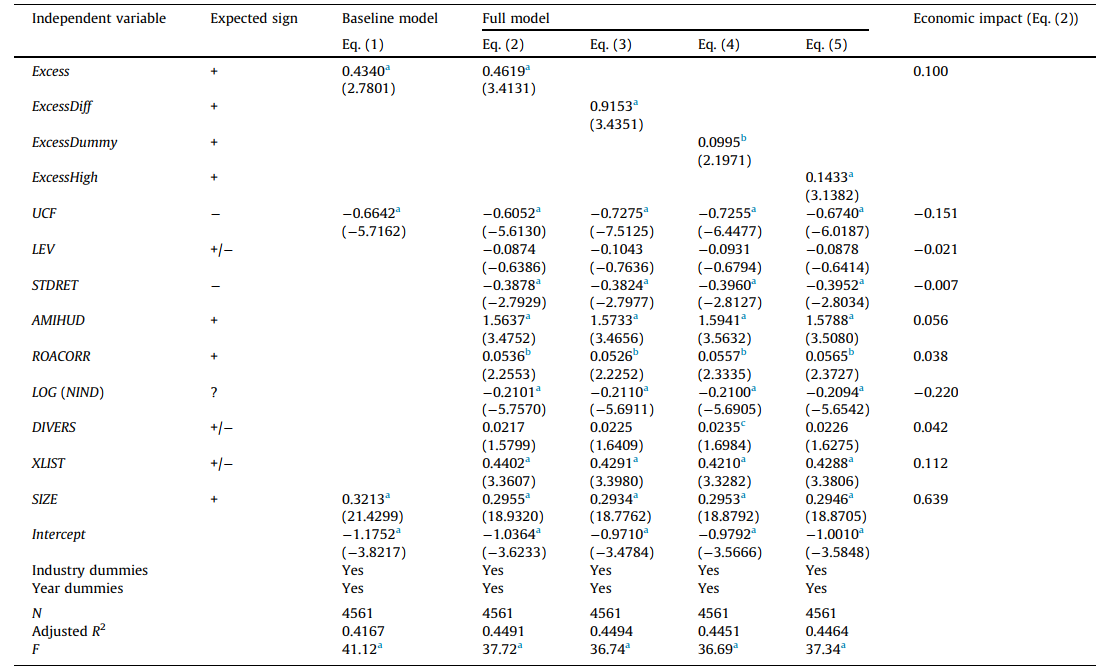
\includegraphics[width=0.9\linewidth]{t4}
	\label{fig:t4}
\end{figure}
\end{frame}
\begin{frame}
			\begin{table}[htbp]
	\centering
	\resizebox{0.75\textheight}{!}{
		{
\def\sym#1{\ifmmode^{#1}\else\(^{#1}\)\fi}
\begin{tabular}{l*{8}{c}}
\hline\hline
                    &\multicolumn{8}{c}{Synchronicity}                                                                                                                                              \\\cmidrule(lr){2-9}
                    &\multicolumn{1}{c}{(1)}         &\multicolumn{1}{c}{(2)}         &\multicolumn{1}{c}{(3)}         &\multicolumn{1}{c}{(4)}         &\multicolumn{1}{c}{(5)}         &\multicolumn{1}{c}{(6)}         &\multicolumn{1}{c}{(7)}         &\multicolumn{1}{c}{(8)}         \\
\hline
Excess              &                     &      -0.899\sym{**} &      -0.557\sym{*}  &                     &                     &                     &                     &                     \\
                    &                     &     [-3.22]         &     [-2.10]         &                     &                     &                     &                     &                     \\
[1em]
ExcessDiff          &                     &                     &                     &      -0.512         &                     &                     &                     &                     \\
                    &                     &                     &                     &     [-1.61]         &                     &                     &                     &                     \\
[1em]
ExcessDummy         &                     &                     &                     &                     &     -0.0900         &                     &                     &                     \\
                    &                     &                     &                     &                     &     [-0.66]         &                     &                     &                     \\
[1em]
ExcessHigh          &                     &                     &                     &                     &                     &      -0.175         &                     &                     \\
                    &                     &                     &                     &                     &                     &     [-1.34]         &                     &                     \\
[1em]
position            &                     &                     &                     &                     &                     &                     &     -0.0959\sym{*}  &                     \\
                    &                     &                     &                     &                     &                     &                     &     [-2.53]         &                     \\
[1em]
centrality          &                     &                     &                     &                     &                     &                     &                     &       1.159\sym{**} \\
                    &                     &                     &                     &                     &                     &                     &                     &      [2.83]         \\
[1em]
cfr                 &                     &      -0.421         &      -0.173         &      0.0838         &       0.244         &       0.102         &       0.119         &       0.336         \\
                    &                     &     [-1.17]         &     [-0.53]         &      [0.31]         &      [0.96]         &      [0.38]         &      [0.50]         &      [1.53]         \\
[1em]
volatility          &    -0.00453         &                     &     -0.0184         &     -0.0168         &     -0.0137         &     -0.0171         &     -0.0182         &     -0.0135         \\
                    &     [-0.27]         &                     &     [-0.95]         &     [-0.87]         &     [-0.69]         &     [-0.86]         &     [-0.92]         &     [-0.69]         \\
[1em]
Liquidity           &      -0.206\sym{***}&                     &      -0.191\sym{***}&      -0.192\sym{***}&      -0.196\sym{***}&      -0.195\sym{***}&      -0.195\sym{***}&      -0.190\sym{***}\\
                    &     [-9.33]         &                     &     [-6.17]         &     [-6.29]         &     [-6.29]         &     [-6.31]         &     [-6.30]         &     [-5.91]         \\
[1em]
Size                &     -0.0873\sym{**} &                     &     -0.0952\sym{*}  &     -0.0917\sym{*}  &     -0.0853\sym{*}  &     -0.0879\sym{*}  &      -0.101\sym{*}  &     -0.0789         \\
                    &     [-3.03]         &                     &     [-2.17]         &     [-2.09]         &     [-2.01]         &     [-2.06]         &     [-2.25]         &     [-1.88]         \\
[1em]
leverage            &      -0.104         &                     &      -0.281\sym{*}  &      -0.291\sym{*}  &      -0.286\sym{*}  &      -0.273\sym{*}  &      -0.334\sym{**} &      -0.199         \\
                    &     [-1.79]         &                     &     [-2.38]         &     [-2.50]         &     [-2.47]         &     [-2.35]         &     [-2.77]         &     [-1.61]         \\
[1em]
 $ \ln(NIND) $      &      -0.138         &                     &      -0.522         &      -0.526         &      -0.567         &      -0.585         &      -0.602         &      -0.396         \\
                    &     [-0.36]         &                     &     [-0.55]         &     [-0.55]         &     [-0.59]         &     [-0.61]         &     [-0.64]         &     [-0.41]         \\
\hline
Industry Dummy      &         Yes         &         Yes         &         Yes         &         Yes         &         Yes         &         Yes         &         Yes         &         Yes         \\
Year Dummy          &         Yes         &         Yes         &         Yes         &         Yes         &         Yes         &         Yes         &         Yes         &         Yes         \\
Observations        &        2550         &        1116         &         978         &         978         &         978         &         978         &         978         &         941         \\
$ R^2 $             &       0.357         &       0.444         &       0.479         &       0.478         &       0.477         &       0.477         &       0.479         &       0.493         \\
\hline\hline
\multicolumn{9}{l}{\footnotesize \textit{t} statistics in brackets}\\
\multicolumn{9}{l}{\footnotesize \sym{*} \(p<0.05\), \sym{**} \(p<0.01\), \sym{***} \(p<0.001\)}\\
\end{tabular}
}

		\label{tab:synchronicityt4}	
	}
\end{table}
\end{frame}

\begin{frame}{Table 5}
	\begin{figure}
		\centering
		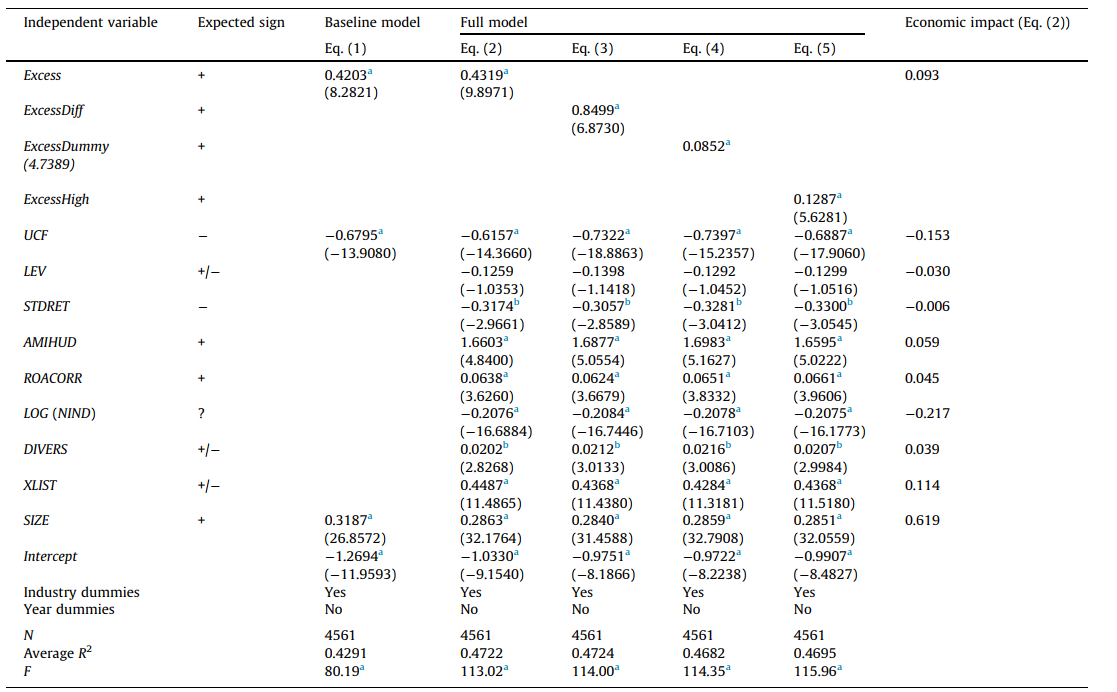
\includegraphics[width=0.9\linewidth]{t5}
		\label{fig:t5}
	\end{figure}
\end{frame}
\begin{frame}
	\begin{table}[htbp]
		\centering
		\resizebox{0.75\textheight}{!}{
			{
\def\sym#1{\ifmmode^{#1}\else\(^{#1}\)\fi}
\begin{tabular}{l*{8}{c}}
\hline\hline
                    &\multicolumn{8}{c}{Synchronicity}                                                                                                                                              \\\cmidrule(lr){2-9}
                    &\multicolumn{1}{c}{(1)}         &\multicolumn{1}{c}{(2)}         &\multicolumn{1}{c}{(3)}         &\multicolumn{1}{c}{(4)}         &\multicolumn{1}{c}{(5)}         &\multicolumn{1}{c}{(6)}         &\multicolumn{1}{c}{(7)}         &\multicolumn{1}{c}{(8)}         \\
\hline
Excess              &                     &      -0.894\sym{**} &      -0.486         &                     &                     &                     &                     &                     \\
                    &                     &     [-4.64]         &     [-2.50]         &                     &                     &                     &                     &                     \\
[1em]
ExcessDiff          &                     &                     &                     &      -0.492         &                     &                     &                     &                     \\
                    &                     &                     &                     &     [-2.05]         &                     &                     &                     &                     \\
[1em]
ExcessDummy         &                     &                     &                     &                     &     -0.0777         &                     &                     &                     \\
                    &                     &                     &                     &                     &     [-1.55]         &                     &                     &                     \\
[1em]
ExcessHigh          &                     &                     &                     &                     &                     &      -0.191         &                     &                     \\
                    &                     &                     &                     &                     &                     &     [-1.73]         &                     &                     \\
[1em]
position            &                     &                     &                     &                     &                     &                     &     -0.0575         &                     \\
                    &                     &                     &                     &                     &                     &                     &     [-2.08]         &                     \\
[1em]
centrality          &                     &                     &                     &                     &                     &                     &                     &       1.497\sym{***}\\
                    &                     &                     &                     &                     &                     &                     &                     &      [7.48]         \\
[1em]
cfr                 &                     &      -0.468         &      -0.269         &     -0.0738         &      0.0783         &      -0.104         &      0.0265         &       0.169         \\
                    &                     &     [-1.58]         &     [-0.79]         &     [-0.25]         &      [0.31]         &     [-0.31]         &      [0.14]         &      [0.81]         \\
[1em]
volatility          &       0.489\sym{**} &                     &       1.654\sym{*}  &       1.616\sym{*}  &       1.615\sym{*}  &       1.686\sym{*}  &       1.657\sym{*}  &       1.580\sym{*}  \\
                    &      [6.17]         &                     &      [2.77]         &      [2.79]         &      [2.79]         &      [2.79]         &      [2.75]         &      [2.83]         \\
[1em]
Liquidity           &      -0.219\sym{***}&                     &      -0.242\sym{***}&      -0.243\sym{***}&      -0.248\sym{***}&      -0.239\sym{***}&      -0.246\sym{***}&      -0.220\sym{***}\\
                    &    [-12.25]         &                     &    [-20.05]         &    [-19.89]         &    [-18.27]         &    [-16.05]         &    [-16.07]         &    [-10.85]         \\
[1em]
Size                &     -0.0910\sym{**} &                     &      -0.126\sym{**} &      -0.125\sym{**} &      -0.115\sym{*}  &      -0.117\sym{*}  &      -0.122\sym{*}  &      -0.101\sym{*}  \\
                    &     [-4.42]         &                     &     [-4.37]         &     [-4.46]         &     [-3.54]         &     [-3.70]         &     [-3.37]         &     [-2.92]         \\
[1em]
leverage            &     -0.0837         &                     &     -0.0894         &     -0.0997         &     -0.0969         &     -0.0835         &      -0.136         &      0.0254         \\
                    &     [-2.31]         &                     &     [-0.52]         &     [-0.59]         &     [-0.58]         &     [-0.47]         &     [-0.82]         &      [0.13]         \\
[1em]
 $ \ln(NIND) $      &      -0.735\sym{**} &                     &      -0.368         &      -0.376         &      -0.593         &      -0.434         &      -0.463         &      -0.398         \\
                    &     [-6.34]         &                     &     [-1.61]         &     [-1.44]         &     [-1.86]         &     [-1.62]         &     [-1.91]         &     [-1.34]         \\
\hline
Industry Dummy      &         Yes         &         Yes         &         Yes         &         Yes         &         Yes         &         Yes         &         Yes         &         Yes         \\
Year Dummy          &          No         &          No         &          No         &          No         &          No         &          No         &          No         &          No         \\
Observations        &        2550         &        1116         &         978         &         978         &         978         &         978         &         978         &         941         \\
$ R^2 $             &       0.327         &       0.462         &       0.547         &       0.547         &       0.544         &       0.546         &       0.550         &       0.568         \\
\hline\hline
\multicolumn{9}{l}{\footnotesize \textit{t} statistics in brackets}\\
\multicolumn{9}{l}{\footnotesize \sym{*} \(p<0.05\), \sym{**} \(p<0.01\), \sym{***} \(p<0.001\)}\\
\end{tabular}
}

			\label{tab:synchronicityt5}	
		}
	\end{table}
\end{frame}

\end{document}